%%
%% Copyright 2007-2020 Elsevier Ltd
%%
%% This file is part of the 'Elsarticle Bundle'.
%% ---------------------------------------------
%%
%% It may be distributed under the conditions of the LaTeX Project Public
%% License, either version 1.2 of this license or (at your option) any
%% later version.  The latest version of this license is in
%%    http://www.latex-project.org/lppl.txt
%% and version 1.2 or later is part of all distributions of LaTeX
%% version 1999/12/01 or later.
%%
%% The list of all files belonging to the 'Elsarticle Bundle' is
%% given in the file `manifest.txt'.
%%
%% Template article for Elsevier's document class `elsarticle'
%% with harvard style bibliographic references

\documentclass[preprint,12pt,authoryear,review]{elsarticle}

%% Use the option review to obtain double line spacing
%% \documentclass[authoryear,preprint,review,12pt]{elsarticle}

%% Use the options 1p,twocolumn; 3p; 3p,twocolumn; 5p; or 5p,twocolumn
%% for a journal layout:
%% \documentclass[final,1p,times,authoryear]{elsarticle}
%% \documentclass[final,1p,times,twocolumn,authoryear]{elsarticle}
%% \documentclass[final,3p,times,authoryear]{elsarticle}
%% \documentclass[final,3p,times,twocolumn,authoryear]{elsarticle}
%% \documentclass[final,5p,times,authoryear]{elsarticle}
%% \documentclass[final,5p,times,twocolumn,authoryear]{elsarticle}

%% For including figures, graphicx.sty has been loaded in
%% elsarticle.cls. If you prefer to use the old commands
%% please give \usepackage{epsfig}

%% The amssymb package provides various useful mathematical symbols
\usepackage{amssymb}
%% The amsthm package provides extended theorem environments
%% \usepackage{amsthm}

% custom
\usepackage{amsmath}
\newcommand*{\norm}[1]{\left\lVert#1\right\rVert}
\newcommand{\argmin}{\arg\!\min}

\usepackage[bottom,hang,flushmargin]{footmisc}

\usepackage[colorlinks]{hyperref}
\hypersetup{citecolor=blue, citebordercolor={1 1 1}}
\usepackage[capitalise]{cleveref}
\usepackage{mathtools}
\usepackage{nth}
\usepackage{siunitx}

%% The lineno packages adds line numbers. Start line numbering with
%% \begin{linenumbers}, end it with \end{linenumbers}. Or switch it on
%% for the whole article with \linenumbers.
%% \usepackage{lineno}
\usepackage{lineno}
\usepackage{color,soul}
\usepackage[dvipsnames]{xcolor}

\usepackage{marginnote}


\journal{NeuroImage}

\begin{document}

    \begin{frontmatter}

        \title{Accelerated Diffusion Weighted Magnetic Resonance Imaging at 7~T: Joint Reconstruction for Multi-Shell Multi-Band Shift-Encoded Echo Planar Imaging (JETS-EPI)
        }

        \author[1]{Zhengguo Tan}
        \author[2]{Patrick Alexander Liebig}
        \author[2]{Robin Martin Heidemann}
        \author[3]{Frederik Bernd Laun}
        \author[1]{Florian Knoll}

        \affiliation[1]{
            organization=Department Artificial Intelligence in Biomedical Engineering (AIBE),
                Friedrich-Alexander-Universität Erlangen-Nürnberg,
            city=Erlangen,
            country=Germany}

        \affiliation[2]{
            organization=Siemens Healthcare GmbH,
            city=Erlangen,
            country=Germany}

        \affiliation[3]{
            organization=Institute of Radiology, University Hospital Erlangen,
                    Friedrich-Alexander-Universität Erlangen-Nürnberg,
            city=Erlangen,
            country=Germany}

        % abstract
        \begin{abstract}
            The pursuit of high spatial-angular-temporal resolution
            for in vivo diffusion-weighted magnetic resonance imaging
            (DW-MRI) at ultra-high field strength (e.g., \SI{7}{\tesla})
            is important in understanding brain microstructure and function.
            Such pursuit, however, faces several technical challenges.
            First, increased off-resonance and shorter $T_2$ relaxation
            require faster echo train readouts.
            Second, high angular resolution in $q$-space requires
            the use of high and/or multiple $b$-values.
            \hl{High \mbox{$b$}-values supply strongly diffusion-weighted images,
            which have lower signal-to-noise ratio (SNR).} \marginnote{R3.13}
            Multi-shot interleaved echo-planar imaging (EPI) and
            advanced reconstruction strategies
            have been proven suitable for high-resolution DW-MRI.
            These methods, however, utilize fully-sampled EPI and thus
            require longer scan time compared to single-shot EPI.
            To address these challenges, \marginnote{R1.6}
            \hl{we developed the \mbox{$k_y$} shift encoding scheme
            among diffusion encodings
            to explore complementary \mbox{$k$}-\mbox{$q$}-space sampling.
            Moreover, we developed a novel joint reconstruction
            with locally low rank regularization}
            for multi-shell multi-band shift-encoding acquisition at \SI{7}{\tesla} (JETS-EPI).
            Our sampling method allows for faster acquisition
            with the use of high in-plane undersampling
            and only two shots per diffusion direction.
            The proposed joint reconstruction exhibits better denoising of DW images
            and clearer delineation of fiber distributions.
            \vspace{3em}
        \end{abstract}

        %%Graphical abstract
        \begin{graphicalabstract}
            \includegraphics[width=\linewidth]{../figures/graph.png}
        \end{graphicalabstract}

        %%Research highlights
        \begin{highlights}
            \item Novel accelerated diffusion acquisition
            with shifted phase encoding among diffusion directions
            for complementary $k$-$q$-space sampling at \SI{7}{\tesla}

            \item Generalized joint $k$-$q$-slice
            diffusion-weighted image reconstruction
            with overlapping locally low-rank regularization

            \item \SI{5}{min} \SI{1.2}{mm} isotropic resolution
            with $b$-value \SI{1000}{s/mm^2} and 32 diffusion directions
            for in vivo whole-brain diffusion tensor imaging

            \item \SI{23}{min} \SI{1}{mm} isotropic resolution
            with three-shell high $b$-values (up to \SI{3000}{s/mm^2})
            and 126 diffusion directions
            for in vivo whole-brain diffusion tensor imaging
            and fiber orientation distribution function (fODF) mapping
            % FL: eventually adapt to what is shown in the paper
        \end{highlights}

        \begin{keyword}
            %% keywords here, in the form: keyword \sep keyword
            Diffusion-weighted magnetic resonance imaging \sep
            Echo planar imaging \sep
            Ultra high field \sep
            Joint reconstruction \sep
            Low rank \sep
            Simultaneous multi slice
        \end{keyword}

    \end{frontmatter}

    \pagebreak
    \linenumbers

    % ************************************************************************ %
    \section{Introduction}
    \label{SEC:Intr}

    Diffusion-weighted magnetic resonance imaging (DW-MRI)
    \citep{lebihan_1986_diff,merboldt_1985_diff} is a non-invasive modality
    that is sensitive to intravoxel Brownian motion of water molecules.
    DW-MRI forms the basis for diffusion tensor imaging (DTI) \citep{basser_1994_dmri,mori_2001_track}
    and high angular resolution diffusion imaging (HARDI) \citep{tuch_2002_hardi},
    and has been widely used in acute brain ischemia diagnosis, in tumor detection and staging,
    and in neuroscience \citep{jones_2010_diff}.

    For DW-MRI acquisition, the commonly used pulse sequence is
    single-shot echo-planar imaging (SS-EPI) \citep{mansfield_1977_epi}.
    SS-EPI is capable of rapidly acquiring one DW image per radio-frequency excitation
    at the order of \SI{100}{\ms}, and is thus motion robust.
    However, conventional SS-EPI,
    even with three-fold accelerated acquisition \citep{bammer_2001_epi_sense}
    using parallel imaging
    \citep{roemer_1990_pi,ra_1993_sense,pruessmann_1999_sense,griswold_2002_grappa},
    still suffers from low spatial resolution and geometric distortions.

    \marginnote{R3.7, R3.8}
    \hl{In the quest for high spatial-angular-temporal-resolution
    and minimal-geometry-distortion DW-MRI,
    tremendous efforts have been made.
    Techniques on the correction of image distortion
    induced by off-resonance and eddy currents
    have been developed \mbox{\citep{andersson_2003_topup}}.
    Furthermore, gSlider \mbox{\citep{setsompop_2018_gslider}} with
    blipped-CAIPI \mbox{\citep{setsompop_2012_blipped}}
    for simultaneous multi-slice (SMS)
    \mbox{\citep{maudsley_1980_sms,breuer_2005_caipi}}
    was proposed to achieve high-resolution DW-MRI.}
    Advanced pulse sequences based on
    \hl{multi-shot EPI} have also been developed, \marginnote{R3.15}
    including but not limited to interleaved EPI \citep{butts_1993_iepi},
    PROPELLER \citep{pipe_2002_blade}, and
    readout-segmented EPI \citep{porter_2009_resolve,heidemann_2010_resolve7t}.
    Based on 4-shot interleaved EPI, advanced image reconstruction techniques,
    e.g.~multiplexed sensitivity encoding (MUSE)
    achieved DW-MRI with sub-millimeter in-plane resolution
    and maximal $b$-value \SI{2000}{s/mm^2} at \SI{3}{\tesla} \citep{chen_2013_muse}.
    In MUSE, four shots (i.e., four-fold undersampling per shot)
    are used because of two reasons.
    First, the high spatial resolution requires the use of multi-shot acquisition,
    which employs a shorter echo train length per shot.
    This allows for reduced echo time and less spatial distortion.
    Second, MUSE employs parallel imaging to reconstruct single-shot images
    for the extraction of shot-to-shot phase variation,
    and four-fold undersampling per shot is achievable in parallel imaging.

    \marginnote{R3.8}
    \hl{Multi-shot EPI, however, prolongs the acquisition time as well as
    introduces motion sensitivity, i.e., shot-to-shot phase variation.}
    Recently, compressed sensing \citep{lustig_2007_cs,block_2007_cs}
    has been explored to accelerate multi-shot EPI acquisition.
    For instance, multi-shot reconstruction techniques
    based on structured low-rank matrix completion (MUSSELS)
    \citep{mani_2017_mussels,bilgic_2019_neatr} achieved
    5-shot DW-MRI with 9-fold undersampling per shot.
    Both MUSSELS and MUSE target the reconstruction of one DW image
    from interleaved EPI using at least 4 shots,
    i.e., joint-$k$-$q$-space undersampling is not explored.

    Joint-$k$-$q$-space undersampling can be achieved via proper regularization
    along the diffusion encoding direction.
    Relevant examples are
    diffusion undersampling with Gaussian process estimated reconstruction (DAGER)
    \citep{wu_2019_dager} and magnitude-based spatial-angular locally low-rank regularization
    (SPA-LLR) \citep{hu_2020_spa_llr}.
    \marginnote{R1.2, R1.10}
    \hl{However, DAGER addresses the reconstruction problem
    of single-shot EPI acquisition.
    SPA-LLR focuses on the reconstruction
    of single-band and in-plane fully-sampled acquisition.}

    In this work, we propose a Joint $k$-$q$-slice rEconsTruction framework
    for multi-band multi-shell Shift-encoded EPI at \SI{7}{\tesla}
    (dubbed as JETS-EPI).
    First, our acquisition method differs from most existing techniques
    as it shifts the $k$-space in-plane sampling pattern
    along the phase encoding ($k_y$) direction.
    This shifting creates complementary $k$-$q$-space sampling.
    Second, our reconstruction framework generalizes to
    jointly reconstruct multi-slice multi-shell multi-direction DW images.
    This is built upon comprehensive modeling of the acquisition process
    and construction of regularization terms (e.g.~LLR) as proximal operators.
    We compared our proposed method with
    state-of-the-art multi-shot reconstruction techniques,
    i.e.,~MUSE and MUSSELS,
    as well as
    \marginnote{R3.20}
    \hl{an established local PCA-based DW image denoising algorithm},
    \citep{manjon_2013_localpca,veraart_2016_denoise}.
    % and Patch2Self \citep{fadnavis_2020_patch2self}.
    Our proposed method achieves \SI{7}{\tesla}
    three-shell high $b$-value (up to \SI{3000}{s/mm^2})
    and 126 diffusion direction measurements
    at \SI{1}{mm} isotropic resolution in less than \SI{23}{min}.

    \clearpage

    % ************************************************************************ %
    \section{Materials and methods}
    \label{SEC:Meth}

    % ============================== %
    \subsection{Multi-band multi-shell shift-encoded EPI acquisition}

    \cref{FIG:sampling} (A) displays diffusion weighted image acquisition
    based on two-shot interleaved EPI.
    Conventionally, such a sampling pattern is repeated for all diffusion directions.
    In contrast, we propose the $k_y$-shifted diffusion encoding,
    as shown in \cref{FIG:sampling} (B).
    The interleaved EPI sampling pattern is shifted by one $k_y$ line
    per diffusion direction,
    with the cycling period being the in-plane undersampling factor.
    \cref{FIG:sampling} (C) displays the employed multi-shell sampling pattern.
    Every diffusion direction is distinct from others,
    thereby constructing a non-colinear sampling pattern.
    This $k_y$-shifted non-colinear diffusion encoding exploits
    complementary $k$-$q$-space sampling. Its properties are two-fold.
    First, the $k_y$-shifting is linear and retains consistent echo spacing.
    Second, DW images share anatomical structures but differ in image contrast
    depending on $b$-values and diffusion directions,
    thus complementary $q$-space sampling is well suited
    for the exploration of structural similarity.
    % FK: I feel you need to motivate why this is beneficial more.
    % FK: This needs more explanation.

    % ============================== %
    \subsection{In vivo acquisition protocols}

    We implemented multiple in-vivo acquisition protocols
    at a clinical \SI{7}{\tesla} MR system
    (MAGNETOM Terra, Siemens Healthineers, Erlangen, Germany)
    equipped with a 32-channel head coil (Nova Medical, Wilmington, MA, USA)
    and the XR-gradient system
    \hl{(maximum gradient strength \mbox{\SI{80}{\milli\tesla / \meter}}
    with a peak slew rate of \mbox{\SI{200}{\tesla / \meter / \second}})}. \marginnote{R3.22}
    To calibrate coil sensitivity maps, reference scans employed a gradient-echo (GRE) sequence.
    Spectral fat saturation and mono-polar diffusion-encoding gradients were used.
    The phase-encoding direction was selected as anterior-to-posterior.

    This study was approved by the local ethics committee. \marginnote{R3.1}
    \hl{Three volunteers with informed consent obtained before scanning
    participated in this study.}
    Detailed acquisition parameters are listed below.

    \subsubsection{20-diffusion-direction 6-shot acquisition
    at \SI{1.0}{\cubic\milli\meter} isotropic resolution
    and $b$-value \SI{1000}{s/mm^2}}
    \label{SEC:ACQ_6shot}

    This protocol employed \SI{200}{\milli\meter} FOV
    in both read and phase-encoding directions,
    base resolution 200, 141 slices, bandwidth \SI{1086}{Hz/Pixel},
    echo spacing \SI{1.06}{ms}, TE \SI{59}{ms}, TR \SI{7600}{ms}.
    Six shots per diffusion encoding with partial Fourier $6/8$
    along the phase-encoding direction was used to
    acquire in-plane full-sampled data.
    In other words, except partial Fourier,
    no in-plane undersampling was used.
    Slice accleration with a multi-band factor $3$ was used.

    \marginnote{R1.1}
    \hl{The acquired data served as ground truth.
    We retrospectively reduced the data to only two shots
    per diffusion encoding with and without the proposed $k_y$ shifting
    to simulate three-fold in-plane undersampling.
    JETS reconstruction was performed on all data to validate
    the proposed two-shot $k_y$-shifted acquisition.}

    \marginnote{R1.2}
    \hl{In addition, different reconstruction methods,
    i.e., JETS, MUSE, and JULEP were performed on the six-shot data
    to validate the JETS reconstruction quality.}

    \subsubsection{Single-shell diffusion acquisition at \hl{\mbox{\SI{1.2}{\cubic\milli\meter} isotropic resolution}}} \marginnote{R1.11}
    \label{SEC:ACQ1.2mm}

    This protocol employed \SI{220}{\milli\meter} FOV in both read and phase-encoding directions,
    base resolution 182, 94 slices, bandwidth \SI{1832}{Hz/Pixel},
    echo spacing \SI{0.75}{ms}, TE \SI{47}{ms}, TR \SI{4300}{ms},
    2 shots per diffusion direction,
    in-plane undersampling $3$ as well as partial Fourier $6/8$ along the phase-encoding direction,
    and multi-band factor $2$. This results in $8.7 \times 2$ fold undersampling per shot.
    30 diffusion directions with $b$-value \SI{1000}{s/mm^2} and
    2 diffusion directions with $b$-value \SI{50}{s/mm^2} were acquired
    at a total scan time of \hl{\mbox{\SI{5.05}{\minute}}}. \marginnote{R3.24}
    Given the high spatial resolution and the short scan time,
    this protocol fits well into clinical studies.

    \subsubsection{Three-shell diffusion acquisition at \hl{\mbox{\SI{1}{\cubic\milli\meter} isotropic resolution}}}
    \label{SEC:ACQ1.0mm}
    This protocol employed the same FOV, shots,
    in-plane undersampling, and partial Fourier as in \cref{SEC:ACQ1.2mm}.
    Other parameters were base resolution 214, 114 slices, bandwidth \SI{1460}{Hz/Pixel},
    echo spacing \SI{0.81}{\milli\second}, TE \SI{66}{\milli\second}, TR \SI{5200}{ms},
    and multi-band factor $3$. This results in $8.7 \times 3$ fold undersampling per shot.
    As shown in \cref{FIG:sampling} (C), three shells were sampled
    (\nth{1} shell: 20 diffusion directions with $b$-value \SI{1000}{s/mm^2},
    \nth{2} shell: 30 diffusion directions with $b$-value \SI{2000}{s/mm^2}, and
    \nth{3} shell: 64 diffusion directions with $b$-value \SI{3000}{s/mm^2}).
    \marginnote{R3.26}
    $b_0$ \hl{acquisitions} were interspersed every ten diffusion directions.
    This corresponds to a total of 126 DW acquisition volumes and
    \hl{\mbox{\SI{22.42}{\minute}}} scan time.
    This protocol will be used to demonstrate the capabilities of JETS-EPI in achieving high
    spatial-angular-temporal resolution.

    \begin{figure}
        \centering
        \includegraphics[width=\linewidth]{../figures/fig1.png}
        \caption{(A) An example DW-MRI acquisition
        with two-shot interleaved EPI acquisition.
        (B) The proposed $k_y$ shifted diffusion encoding scheme.
        This example employs two shots per DW image.
        Therefore, every two columns have the same color.
        (C) An example multi-shell sampling scheme.
        (D) Low rankness of local image patches (as extracted from the yellow blocks)
        along multi-shell diffusion encoding.}
        \label{FIG:sampling}
    \end{figure}

    \pagebreak

    % ============================== %
    \subsection{Forward modeling}
    Our proposed acquisition method yields multi-dimensional but
    slice collapsed $k$-space data $\mathbf{y}_{c,q,s}$,
    where $c$, $q$, $s$ denotes the index of the coil sensitivity map,
    the diffusion encoding, and the shot, respectively.
    Acquisition modeling needs to consider several aspects.

    First, the acquired $k$-space data $\mathbf{y}$ is mapped from
    individual shot images $\mathbf{x}_{q,s,z}$ via the forward model,
    \begin{align}
        \mathbf{y}_{c,q,s} &= \mathbf{P}_{q,s} \mathbf{\Sigma} \mathbf{\Theta}_{z} \mathbf{F} \mathbf{S}_c \mathbf{x}_{q,s,z} \\
        \mathbf{y} &\coloneqq \mathbf{E}_1 \mathbf{x} \label{EQU:model_shot}
    \end{align}
    Here, the encoding matrix $\mathbf{E}_1$ comprises a chain of linear operators.
    Every shot image $\mathbf{x}$ is point-wise multiplied
    by a set of coil sensitivity maps ($\mathbf{S}$) and Fourier transformed ($\mathbf{F}$).
    The output is then point-wise multiplied by the multi-slice phase map ($\mathbf{\Theta}$)
    with $z$ the slice index in simultaneously excited slices.
    This operator shifts individual slice along the phase-encoding direction
    via varying phase modulation \citep{breuer_2005_caipi}.
    The SMS $k$-space data is then
    summed (collapsed, $\mathbf{\Sigma}$) along the slice dimension and
    masked (point-wise multiplied, $\mathbf{P}$) by
    the sampling pattern of each diffusion encoding and shot.

    Second, for diffusion MRI based on multi-shot EPI,
    multiple shots acquired for a given diffusion encoding
    need to be combined as one DW image ($\mathbf{\tilde{x}}$).
    A possibility is to perform magnitude average \citep{chen_2013_muse}
    or root-sum-squares (RSS) \citep{mani_2017_mussels}
    of shot images.
    This method is robust to \hl{in-plane} motion, \marginnote{R3.27}
    but sub-optimal with respect to SNR
    \citep{guhaniyogi_2016_amuse}.
    Alternatively, shot combination can be done via shot-to-shot phase variation correction
    \citep{liu_2005_moco_diff,chen_2013_muse}.
    This can be incorporated to our formulation as point-wise multiplication
    between the shot-to-shot phase variation ($\mathbf{\Phi}$) and
    % FK: Can you explain how $\mathbf{\Phi}$ is obtained during the measurement?
    the DW image ($\mathbf{\tilde{x}}$),
    \begin{equation}
         \mathbf{x}_{q,s,z} = \mathbf{\Phi}_{q,s,z} \mathbf{\tilde{x}}_{q,z}
    \end{equation}
    Note that $\mathbf{\tilde{x}}$ can be obtained
    by applying the adjoint of $\mathbf{\Phi}$ to $\mathbf{x}$.
    In MUSE, $\mathbf{\Phi}$ is obtained by parallel imaging reconstruction of all shots
    with subsequent phase smoothing of every shot image.
    Based on this phase correction, the complete forward model follows
    \begin{equation}
        \mathbf{y} \coloneqq \mathbf{E}_2 \mathbf{\tilde{x}} = \mathbf{E}_1 \mathbf{\Phi} \mathbf{\tilde{x}}
        \label{EQU:model_dwi}
    \end{equation}
    where the encoding matrix $\mathbf{E}_2$ comprises the chain of
    the shot-to-shot phase variation $\mathbf{\Phi}$ and
    the encoding matrix $\mathbf{E}_1$.
    We implemented these two encoding matrices in SigPy \citep{ong_2019_sigpy}.


    % ============================== %
    \subsection{Joint $k$-$q$-slice reconstruction}

    Based on the generalized forward models in \cref{EQU:model_shot,EQU:model_dwi},
    our proposed joint $k$-$q$-slice reconstruction can be formulated as a three-step approach.

    \begin{enumerate}[I.]
        \item Joint reconstruction of all shot images
        by solving the following inverse problem with
        the LLR regularization:
        \begin{equation}
            \mathrm{argmin}_\mathbf{x} \left\| \mathbf{y} - \mathbf{E}_1 \mathbf{x} \right\|_2^2
            + \lambda \left\| \mathbf{T} \mathbf{x} \right\|_*
            \label{EQU:solve_shot}
        \end{equation}
            Note that this step suffices in the case of single-shot EPI acquisition.

        \item For multi-shot EPI acquisition,
        shot-to-shot phase variation is extracted from $\mathbf{x}$.
        \marginnote{R1.13}
        \hl{Assuming that phase images are spatially smooth}
        \citep{chen_2013_muse,dai_2023_julep},
        only the central quarter $k$-space region of $\mathbf{y}$
        is used to solve for $\mathbf{x}$.
        Afterward, the reconstructed $\mathbf{x}$ is interpolated to the full FOV.
        The corresponding phase is then filtered by the Hanning window.

        \item Joint reconstruction of all DW images using
        the shot-combined forward model $\mathbf{E}_2$
        with shot-to-shot phase variation from Step II:
        \begin{equation}
            \mathrm{argmin}_\mathbf{\tilde{x}} \left\| \mathbf{y} - \mathbf{E}_2 \mathbf{\tilde{x}} \right\|_2^2
            + \lambda \left\| \mathbf{T} \mathbf{\tilde{x}} \right\|_*
            \label{EQU:solve_dwi}
        \end{equation}
    \end{enumerate}

    % ============================== %
    \subsection{Locally low rank (LLR) regularization}

        % FK: I feel you need to motivate more why the matrix has low rank than just showing a plot of a single example
    As shown in \cref{FIG:sampling} (D), low rankness exists
    in local patches from multi-shell DW images.
    Intuitively, low rankness comes from the contrast variation feature of DW images.
    This motivates the application of LLR regularization \citep{trzasko_2011_lr,zhang_2015_llr}
    for solving the inverse problems in \cref{EQU:solve_shot,EQU:solve_dwi}.
    Here, $\lambda$ is the regularization strength ($\lambda \geq 0$).
    $\mathbf{T}$ represents a linear operator that firstly slides a local patch window
    through all DW images and then
    flattens every set of local patches to two-dimensional (2D) matrices.
    The nuclear norm regularization is enforced via
        singular value thresholding of all flattened 2D matrices \citep{cai_2010_svt}.
    We implemented this regularization term as \hl{a proximal operator}
    \citep{beck_2017_optim}. \marginnote{R3.28}

    It has been reported that LLR is prone to checkerboard artifacts
    when $\lambda$ is too large \citep{hu_2020_spa_llr}.
    We overcome this problem by utilizing overlapping blocks and providing an efficient implementation.
    If the blocks overlap, $\mathbf{T}^H \mathbf{T}~\mathrm{input} \neq \mathrm{input}$,\marginnote{R3.30}
    where $\mathbf{T}^H$ denotes the \hl{Hermitian} adjoint operator of $\mathbf{T}$.
    Our efficient implementation is to scale $\mathbf{T}^H$
    as $(1 / \mathrm{divisor})\mathbf{T}^H$,
    where the divisor matrix is obtained by $\mathbf{T}^H \mathbf{T}~\mathbf{1}$.
    $\mathbf{1}$ denotes the matrix of ones with the same shape as \hl{the input}. \marginnote{R3.31}

    % ============================== %
    \subsection{Reconstruction}

    The acquired raw data was read in by twixtools
    (\url{https://github.com/pehses/twixtools}).
    Ramp-sampling regridding and FOV/2-ghost correction were also performed in twixtools.
    Subsequently, coil sensitivity maps were computed from reference scans
    using ESPIRiT \citep{uecker_2014_espirit} in SigPy \citep{ong_2019_sigpy}.

    With this pre-processing as well as
    the implemented forward models and proximal operator,
    both inverse problems in \cref{EQU:solve_shot,EQU:solve_dwi} were solved by
    the alternating direction method of multipliers (ADMM) \citep{boyd_2010_admm}.

    ADMM solves the minimization problems in an alternating update scheme,
    \begin{equation}
        \left\{\begin{matrix}
            \begin{aligned}
                \mathbf{x}^{(k+1)} &:= \argmin_{\mathbf{x}} \norm{\mathbf{y} - \mathbf{E}(\mathbf{x})}^2 + \rho/2 \norm{\mathbf{T}\mathbf{x} - \mathbf{z}^{(k)} + \mathbf{u}^{(k)}}_2^2 \\
                \mathbf{z}^{(k+1)} &:= \mathcal{T}_{\lambda/\rho} (\mathbf{T} \mathbf{x}^{(k+1)} + \mathbf{u}^{(k)}) \\
                \mathbf{u}^{(k+1)} &:= \mathbf{u}^{(k)} + \mathbf{T} \mathbf{x}^{(k+1)} - \mathbf{z}^{(k+1)}
            \end{aligned}
        \end{matrix}\right.
        \label{EQU:ADMM}
    \end{equation}
    where $k$ denotes the ADMM iteration.
    $\mathbf{z}$ is the auxiliary variable ($\mathbf{z} = \mathbf{T}\mathbf{x}$),
    and $\textbf{u}$ is the Lagrangian multipliers.
    Importantly, when solving \cref{EQU:model_shot},
    $\textbf{x}$ denotes shot images and $\mathbf{E}$ denotes $\mathbf{E}_1$ in \cref{EQU:ADMM}.
    In contrast, $\textbf{x}$ denotes shot-combined images and $\mathbf{E}$ denotes $\mathbf{E}_2$
    when solving \cref{EQU:model_dwi}.
    $\mathbf{x}$ can be solved using linear least square algorithms, \marginnote{R3.35}
    e.g.~conjugate \hl{gradients} \citep{hestenes_1952_cg},
    \marginnote{R2.8, R3.32}
    while $\mathbf{z}$ is updated via \hl{singular value thresholding
    (\mbox{$\mathcal{T}$}) with the thresholding parameter \mbox{$\lambda / \rho$}}.
    The coupling parameter $\rho$ is effective in both the update of $\mathbf{x}$ and $\mathbf{z}$.
    It acts as Tikhonov regularization strength when updating $\mathbf{x}$,
    but also inversely scales the thresholding strength when updating $\mathbf{z}$,
    as shown in Supporting Information Figures S1 and S2.

    In this work, 15 ADMM iterations with $\rho = 0.05$ and $\lambda = 0.04$,
    and a block size of 6 for LLR (refer to Supporting Information Figure S3)
    were used.
    All reconstructions were done on a single A100 SXM4/\hl{NVLink} GPU \marginnote{R3.37}
    with \SI{40}{GB} memory (NVIDIA, Santa Clara, CA, USA).

    We compared our proposed joint reconstruction
    with established multi-shot reconstruction techniques,
    specifically, MUSE \citep{chen_2013_muse},
    MUSSELS \citep{bilgic_2019_neatr},
    and JULEP \citep{dai_2023_julep}.
    \marginnote{R1.3}
    \hl{Here, MUSE and JULEP are hosted on GitHub by Dr.~Dai,
    and MUSSELS with the multi-band reconstruction feature
    is made available by Dr.~Bilgic.
    Further, we performed
    the local-PCA denoising \mbox{\citep{manjon_2013_localpca}}
    as implemented in DIPY \mbox{\citep{garyfallidis_2014_dipy}}
    on the MUSE reconstructed DW images.}

    With reconstructed DW images, fractional anisotropy (FA) maps
    \citep{basser_1994_dmri} were fitted using our implementation in Python,
    whereas fiber orientation distribution functions (fODF)
    \citep{aganj_2009_solidangle}
    were computed in MITK-Diffusion \citep{fritzsche_2012_mitk_diff}
    with the spherical harmonic order \num{4} and the regularization factor \num{0.002}.
    fODF maps were displayed with the min-max normalization
    \marginnote{R3.41}
    and the FA/GFA \hl{(generalized fractional anisotropy)}
    scaling factor \num{2.2}.

    \pagebreak

    % ************************************************************************ %
    \section{Results}
    \label{SEC_Resl}

    \subsection{\hl{Validation of the proposed two-shot EPI acquisition via retrospectively undersampling from a six-shot EPI acquisition}}
    \marginnote{R1.1}

    JETS reconstruction results on
    the six-shot prospectively fully-sampled data
    from the acquisition protocol in \cref{SEC:ACQ_6shot},
    as well as on the retrospectively undersampled two-shot data
    without and with the proposed $k_y$ shift
    are displayed in \cref{FIG:gt_6shot}.
    Noticeable signal loss can be observed in the 2-shot reconstruction
    without $k_y$ shift, as indicated by red arrows.
    In contrast, the visible difference between the 6-shot and
    the $k_y$-shifted 2-shot reconstructions is smaller,
    especially in the averged DW image.
    This is also confirmed with the quantitative comparison
    of the normalized root mean square error (NRMSE),
    as listed in the bottom right of difference images.
    The NRMSE values are lower in the reconstruction
    with $k_y$ shifting,
    indicating a closer match with the 6-shot reconstruction.



    % \subsection{Single-shell diffusion acquisition at \SI{1.2}{\milli\meter} isotropic resolution}

    % \cref{FIG:1.2mm_DWI_cFA} displays a DW image
    % for one diffusion direction and zoomed-in colored FA maps from
    % MUSE, MUSE with denoising, MUSSELS, and JETS reconstruction.
    % Both MUSE and MUSSELS exhibit residual noise artifacts
    % for the single-shell acquisition with the $b$-value of \SI{1000}{s/mm^2}.
    % The local PCA denoiser removes noise, but the denoised DW image loses fine structures,
    % e.g.~the~cuneus (highlighted by the arrows in the figure).
    % This over-smoothing effect can also be observed in the colored FA map,
    % where the thin fibers near to gray matter are missing.

    \begin{figure}
        \centering
        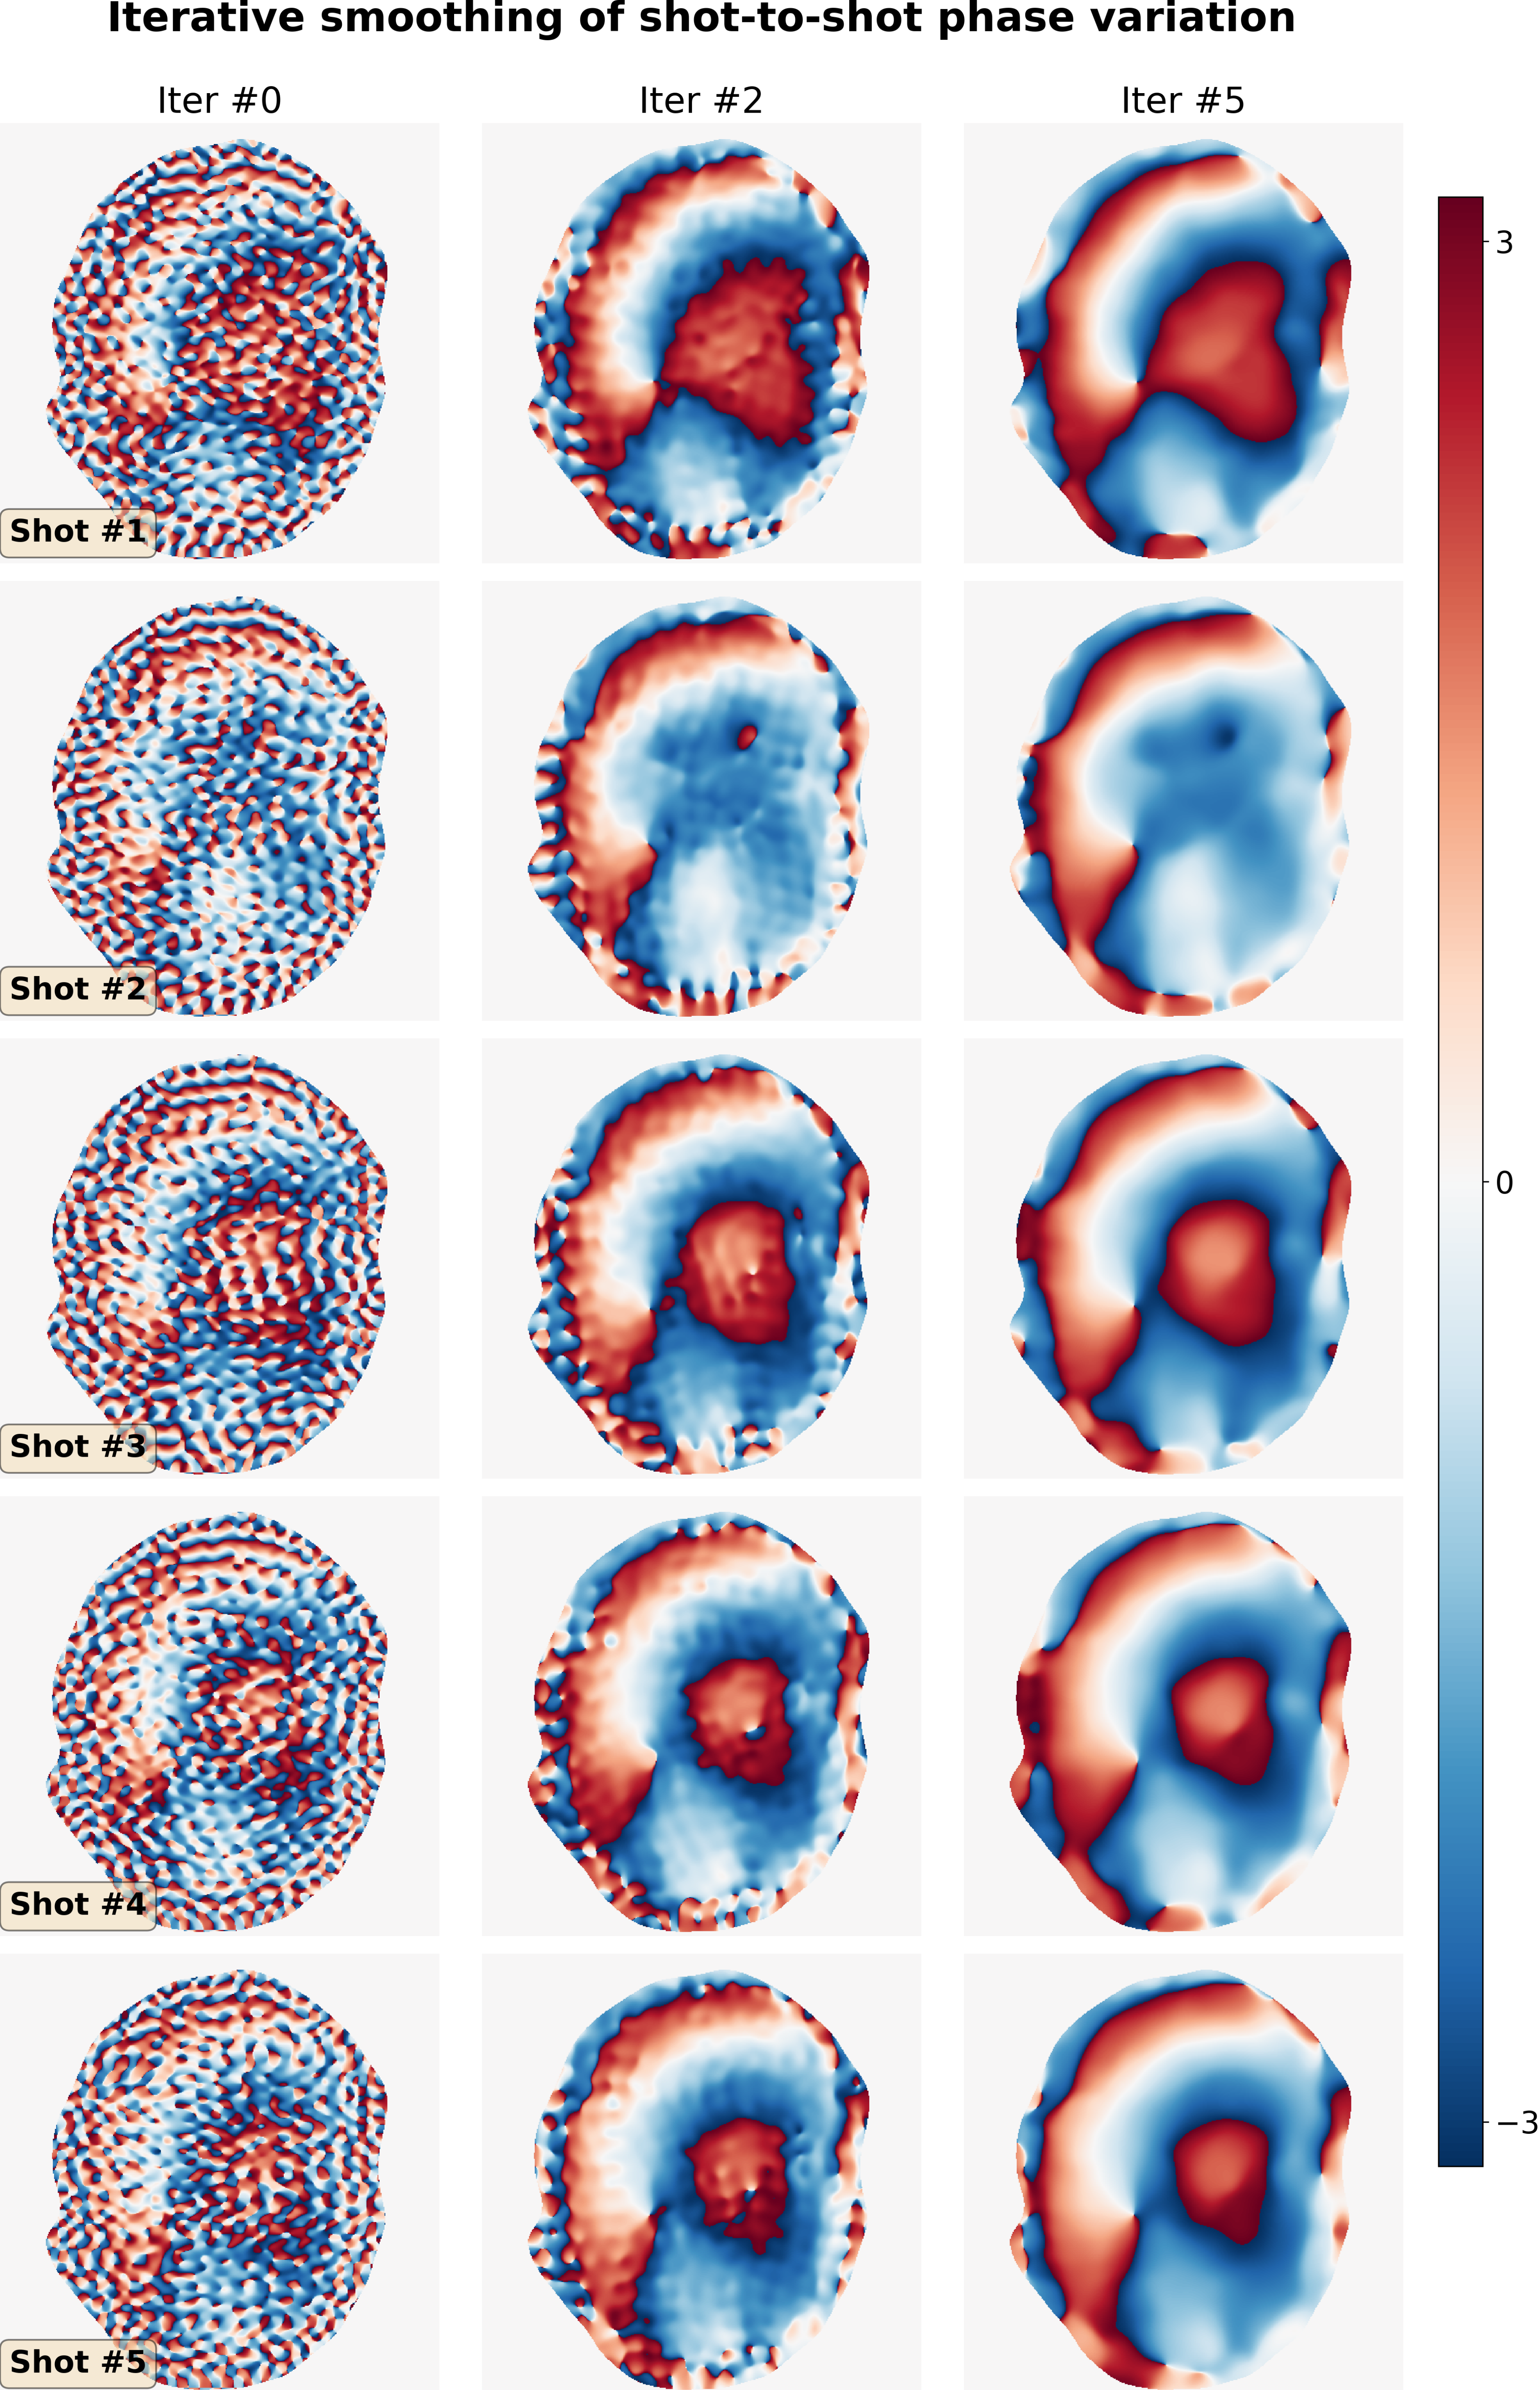
\includegraphics[width=0.85\linewidth]{../figures/fig2.png}
        \caption{\protect\marginnote{R1.1}[0cm]
            JETS reconstruction results on
            (1st column) the 6-shot sampled data from \cref{SEC:ACQ_6shot},
            the retrospectively undersampled 2-shot data
            (2nd column) without $k_y$ shift as well as
            (3rd column) with $k_y$ shift.
            Difference images were obtained by
            subtracting the 6-shot from
            the 2-shot reconstructed images.
            \textbf{(A)} and \textbf{(B)} display
            the 8th DW and the averaged DW images,
            respectively.}
        \label{FIG:gt_6shot}
    \end{figure}


    \subsection{Three-shell diffusion acquisition at \SI{1.0}{\milli\meter} isotropic resolution}

    Results for a \SI{1.0}{mm} isotropic resolution three-shell 126-direction
    diffusion acquisition are show in \cref{FIG:1.0mm_DWI}.
    At this resolution, a severe reduction of SNR can be observed
    for higher $b$-values.
    With such low SNR levels, brain structures are completely buried below the noise level
    in MUSE and MUSSELS.
    The local PCA denoiser removes noise efficiently from the reconstructed MUSE images,
    but images from higher $b$-values suffer from severe blurring that leads to
    a loss of fine image details.
    Only the proposed JETS method with the combination of the $k_y$-shift encoding scheme
    and LLR regularized reconstruction allows for the resolution of brain features for higher $b$-values.

    \begin{figure}
        \centering
        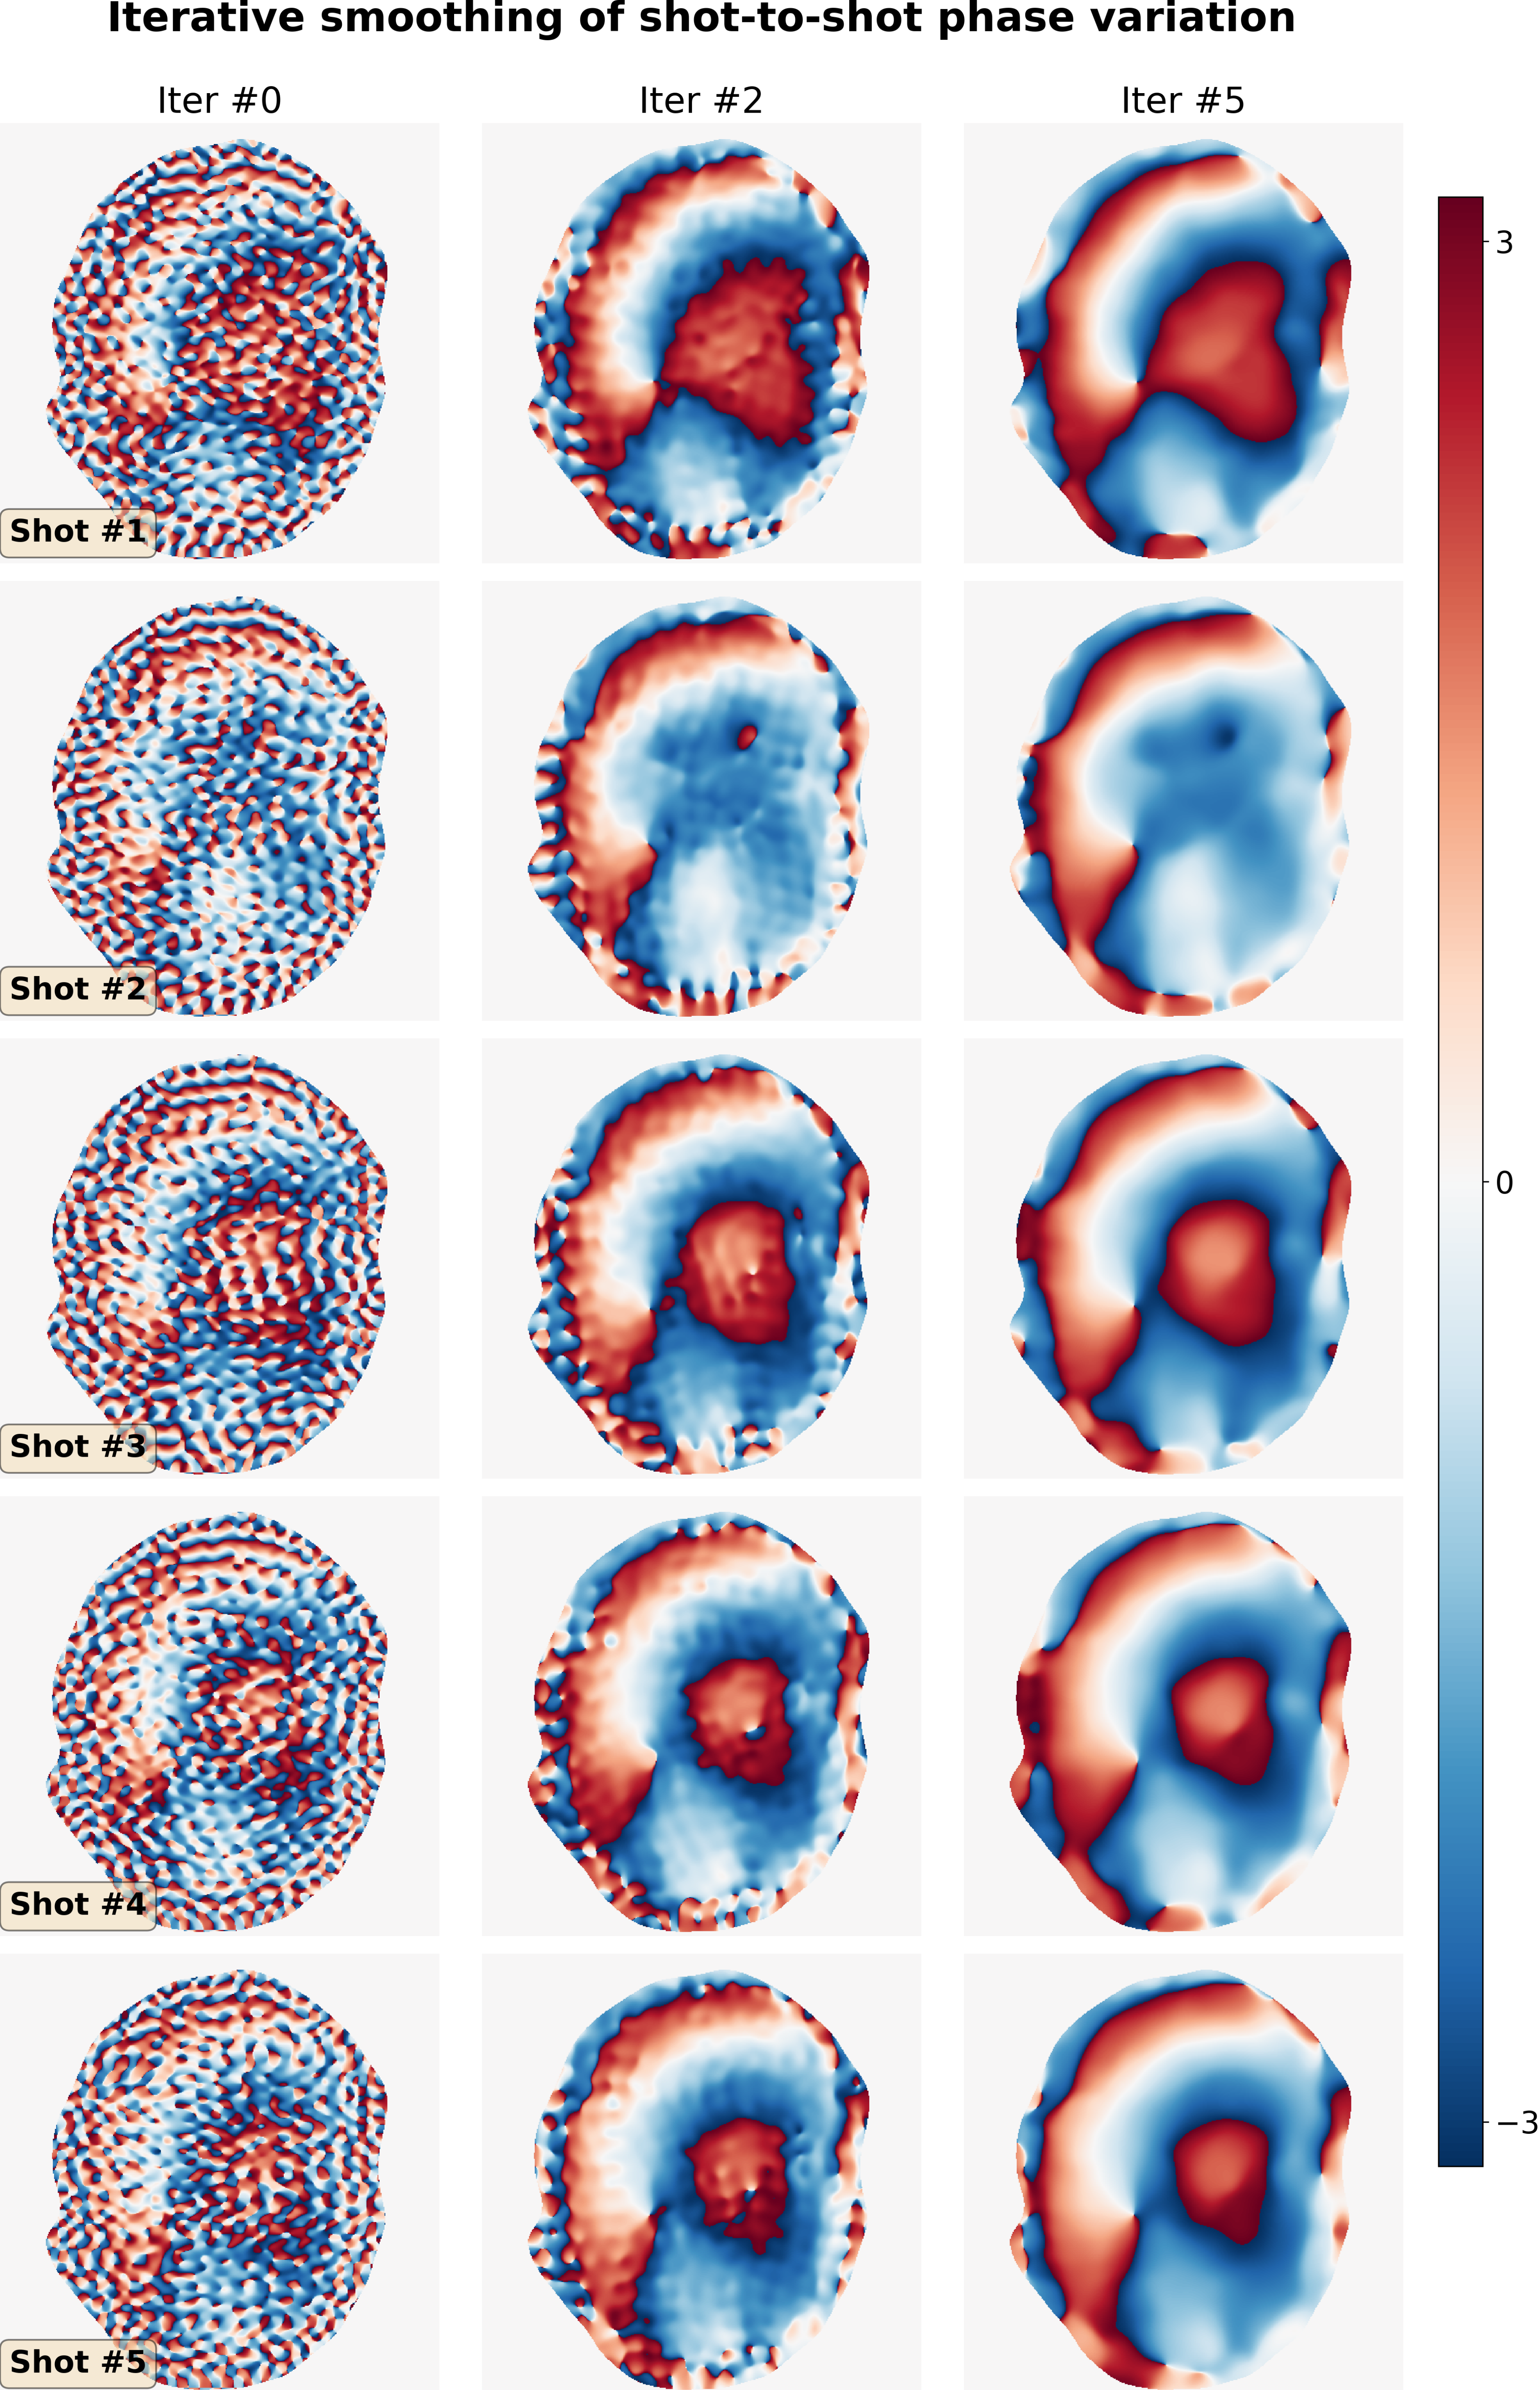
\includegraphics[width=\textwidth]{../figures/fig3.png}
        \caption{Comparison of reconstructed DW images on
            three-shell diffusion acquisition at
            \SI{1}{\milli\meter} isotropic resolution.
            DW images of the \nth{60} slice for one diffusion direction at different $b$-values are displayed:
                (left) 1000, (center) 2000, and (right) 3000~\si{s/mm^2}.}
        \label{FIG:1.0mm_DWI}
    \end{figure}

    \cref{FIG:1.0mm_FA} shows fitted FA maps
    in three orthogonal orientations
    based on the above four DW image reconstruction methods.
    Corresponding color-coded FA maps are provided
    in Supporting Information Figure S6.
    % (Although DW images are noisy from both MUSE and MUSSELS,
    % parameter fitting (e.g., FA) reduces noise in the fitted maps.
    % FK: I am not sure we should make this statement. Doesn't this mean that we are simply seeing fits where the high-b-value information is lost, because the diffusion information is below the noise level? So the FA maps may look better visually than the DWIs, but they still contain less information)
    All FA maps are displayed with the same windowing,
    i.e., minimal and maximal values set as 0 and 1, respectively.
    The FA maps from MUSE with local PCA denoising
    exhibit much lower values than other methods.
    This may be caused by the excessive noise in DW images from MUSE
    or by the automatic noise estimate in the local PCA denoising algorithm
    \citep{veraart_2016_denoise}.
    Among all methods, FA maps from JETS show better quality
    and delineate fine details within the putamen (see white arrows).

    \begin{figure}
        \centering
        \includegraphics[width=0.85\textwidth]{../figures/fig4.png}
        \caption{Comparison of reconstructed FA maps based on
            the \SI{1}{mm} isotropic resolution
        three-shell diffusion acquisition.
        One slice from every orientation
        (axial, coronal, and sagittal view from left to right)
        was selected for display.}
        \label{FIG:1.0mm_FA}
    \end{figure}

    \cref{FIG:1.0mm_fODF} shows fODF maps
        within the rectangular regions in \cref{FIG:1.0mm_FA}.
        This result again demonstrates
        the advantage of iterative reconstruction with LLR regularization
        for DW image denoising.
        Both MUSE and MUSSELS reconstructions suffer from noise artifacts due to
        the use of highly accelerated acquisition ($R = 8.7 \times 3$ per shot)
        and high $b$-values (up to \SI{3000}{s/mm^2}).
        As a result, their corresponding fODF maps illustrate chaotic fiber orientation.
        With the local PCA denoiser applied to DW images reconstructed by MUSE,
        the fODF peaks show improved smoothness, but the FA values are reduced
        due to excessive noise in DW images.
        In contrast, with LLR regularization applied to
        the \hl{spatial-diffusion} patches, \marginnote{R1.45}
        JETS is able to resolve crossing fibers in the intersection of corpus callosum
        and superior longitudinal fasciculus (see white arrows).

    \begin{figure}
        \centering
        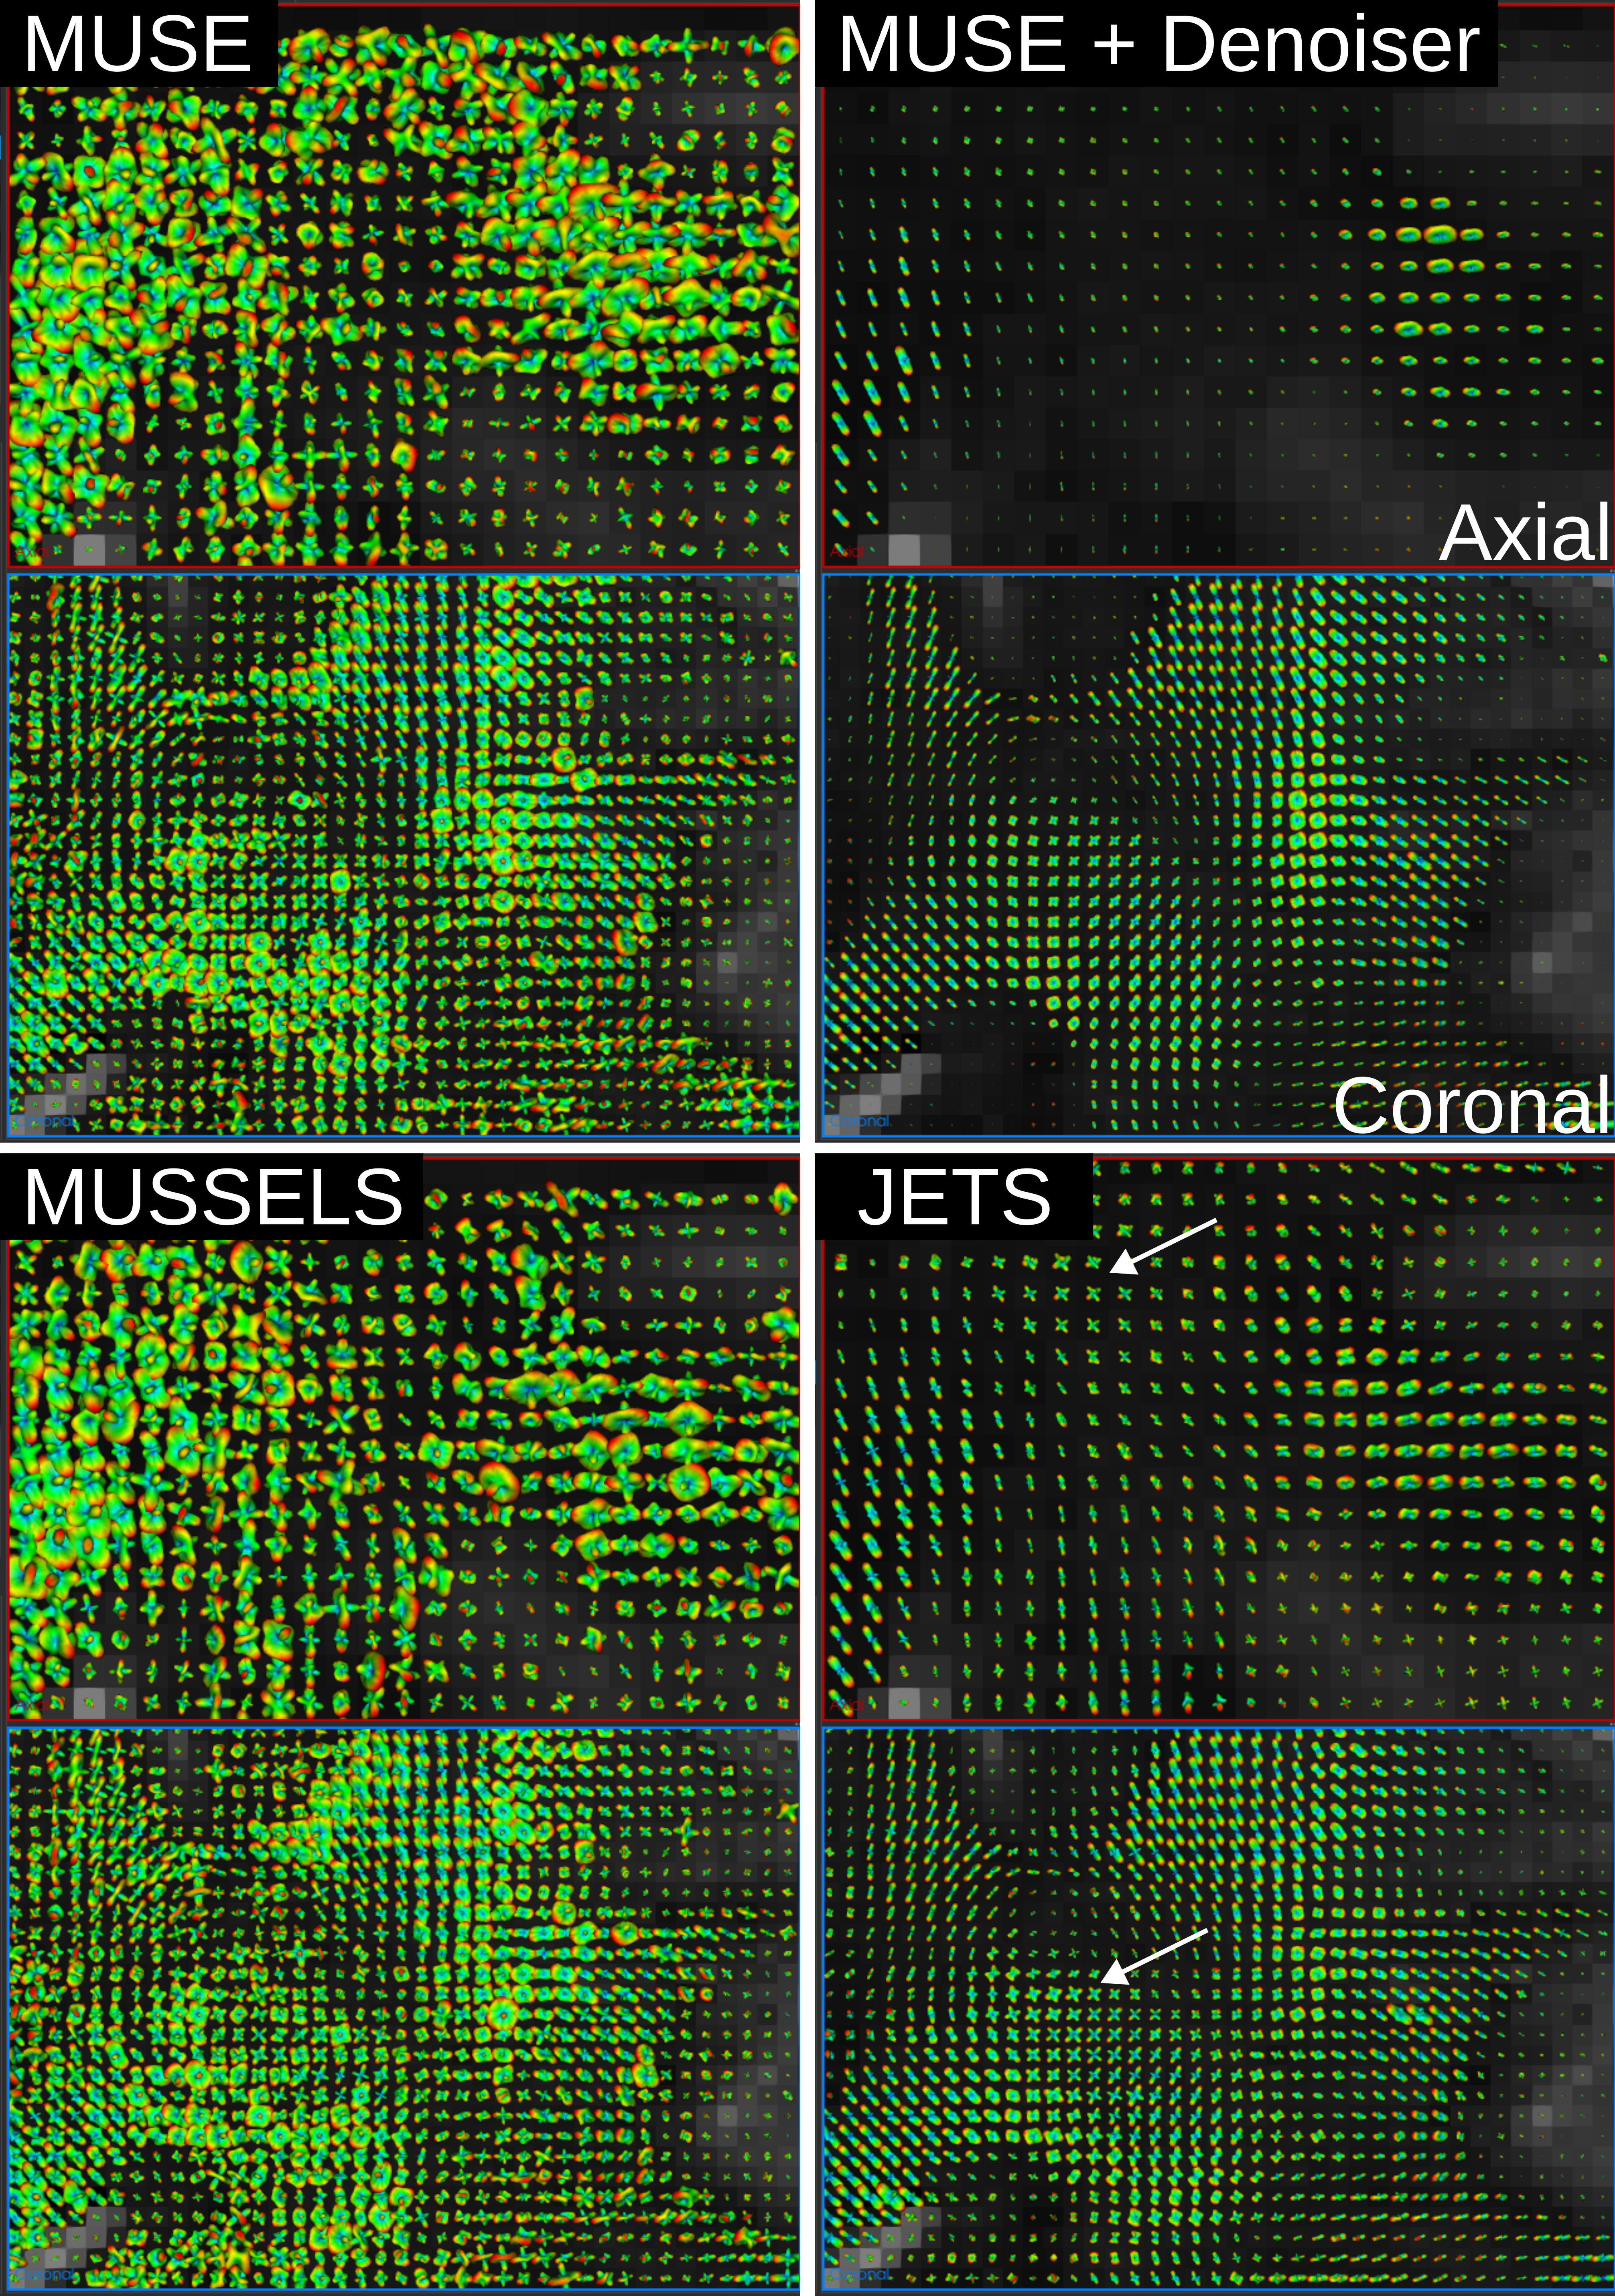
\includegraphics[width=0.9\textwidth]{../figures/fig5.png}
        \caption{Comparison of fODF peaks within the dashed rectangles
        of (red) the axial and (blue) the coronal slices in \cref{FIG:1.0mm_FA}, respectively.}
        \label{FIG:1.0mm_fODF}
    \end{figure}

    \clearpage

    % ************************************************************************ %
    \section{Discussion}
    \label{SEC:Disc}

    This work reports a novel DW-MRI technique, \hl{dubbed JETS-EPI}, \marginnote{R3.45}
    comprising two ingredients,
    multi-band $k_y$-shift-encoded interleaved EPI
    for complementary $k$-$q$-space sampling, and
    a generalized joint reconstruction
    with overlapping locally low-rank regularization
    to explore low rankness along the diffusion encoding dimension.
    JETS-EPI utilizes only two shots \hl{per diffusion-weighted image}, \marginnote{R3.46}
    thereby allowing for short scan times
    as well as high spatial resolution with reduced geometric distortion.
    Our reconstruction uses $8.7 \times 3$ ($R_\mathrm{in-plane} \times \mathrm{SMS}$)
    fold accelerated brain DW-MRI at \SI{7}{\tesla}
    with \SI{1}{mm} isotropic resolution
    and 126 diffusion-direction (three shells with
    $b$-values of $1000$, $2000$, and \SI{3000}{s/mm^2})
    in less than \SI{23}{min}.
    % (FK: This is more or less a repetition of the results section. We should discuss here what the reason for the improved performance is)

    The reconstruction results from MUSE and MUSSELS
    suffer from noise effects in this study,
    and the reasons are two-fold.
    First, the high in-plane undersampling factor per shot
    hinders shot-to-shot phase variation estimation in MUSE,
    whereas we proposed to jointly reconstruct all shot images from the central $k$-space data.
    Further, joint reconstruction benefits from the complementary $k$-$q$-space sampling,
    as compared to the shot-by-shot parallel imaging reconstruction.
    Second, structured low-rank matrix completion as \hl{used by} MUSSELS usually \marginnote{R3.47}
    works with at least four shots per diffusion direction,
    whereas this study uses only two shots.
    The use of two shots is beneficial for shorter scan time than four shots,
    but hinders the structured low rank property in MUSSELS.

    One limitation of JETS-EPI is the long reconstruction time
    due to the simultaneous reconstruction of all DW images and
    the use of overlapping locally low-rank regularization.
    The reconstruction of the protocols in \cref{SEC:ACQ1.2mm} and \cref{SEC:ACQ1.0mm} \marginnote{R3.48}
    \hl{on an A100 GPU} takes about \SI{0.5}{\hour} and \SI{3}{\hour} per collapsed slice, respectively.
    To reduce the computation time, coil compression algorithms \citep{huang_2008_scc}
    can be employed to reduce the number of coils for image reconstruction.
    Moreover, one may deploy multi-GPU distributed computing or modern optimization algorithms
    (e.g.~stochastic gradient descent) \citep{ong_2020_extreme} to speed up the reconstruction.

    Another limitation of JETS-EPI is the self-navigated shot-to-shot phase variation estimation,
    which was performed based on the central quarter $k$-space region of every shot.
    These shot $k$-space data is highly undersampled with $R = 8.7 \times 3$
    for the \SI{1}{mm} three-shell diffusion acquisition.
    Such high undersampling may result in sub-optimal phase estimation,
    especially in regions with low SNR and/or rapid phase change.

    \marginnote{R1.5, R3.2}
    \hl{To be discussed: LLR regularization performance and reliability may degrade in the presence of motion. Also, often DWI is performed with alternating PEs for distortion correction. SNR is heterogeneous over the FOV, which may not be appropriately covered by a single regularization weight. Please, add these aspects to discussion. See also minor point 5.}

    \marginnote{R1.13}
    \hl{Discussion on phase: Think you should add a bit more on this topic to discussion, as phase behaviour depends on several hard-to-control factors such as pulsatile motion, its impact at different locations within the brain, diffusion sensitization strength, bulk motion, ...}



    While this work reconstructs all DW images and then performs model fitting,
    an alternative approach is to directly estimate $b_0$ and diffusion tensors
    from measured $k$-$q$-space data using model-based reconstruction
    \citep{knoll_2015_mobadiff,dong_2018_mobadiff,shafieizargar_2023_adept}.
    Compared to DW image reconstruction,
    model-based reconstruction \hl{solves for a fewer number of unknowns}, \marginnote{R3.49}
    but requires strict diffusion tensor modeling and the use of nonlinear least square solvers.

    % ************************************************************************ %
    \section{Conclusions}
    \label{SEC:Conc}

    We demonstrated the JETS-EPI technique, which integrates
    a $k_y$-shifted encoding interleaved EPI sequence and
    a joint reconstruction with overlapping locally low-rank regularization
    for high spatial-angular-temporal resolution DW-MRI at \SI{7}{\tesla}.
    This technique requires no phase navigation,
    and allows for high-quality DW image reconstruction with accelerated acquisitions.

    % ************************************************************************ %
    \section*{Funding}

    This work was supported by Deutsche Forschungsgemeinschaft (DFG) -- Project Number 513220538,
    as well as National Institutes of Health (NIH) R01 EB024532 and P41 EB017183.

    % ************************************************************************ %
    \section*{Data and code available statement}

    In the spirit of reproducible and open science,
    we will publish our source code ({\url{https://github.com/ZhengguoTan/sigpy})
    as well as the raw $k$-space data ({\url{https://doi.org/10.5281/zenodo.7548595})
    during the review process.

    % ************************************************************************ %
    \section*{Acknowledgments}
        The authors thank Dr.~Peter Neher for the discussion on MITK-Diffusion.
        % https://hpc.fau.de/faqs/#innerID-1437
        The authors gratefully acknowledge the scientific support and HPC resources
        provided by the Erlangen National High Performance Computing Center (NHR@FAU)
        of Friedrich-Alexander-Universit\"at Erlangen-N\"urnberg (FAU)
        under the NHR project b143dc.
        NHR funding is provided by federal and Bavarian state authorities.
        NHR@FAU hardware is partially funded by the German Research Foundation (DFG) -- 440719683.

        \marginnote{R1.2}
        The authors thank
        \hl{Dr.~Berkin Bilgic} for making the MUSSELS source code
        (\url{https://bit.ly/2QgBg9U}) publically available,
        \hl{Dr.~Erpeng Dai} for sharing the JULEP source code
        (\url{https://github.com/daiep/JULEP}) on GitHub,
        and \hl{Dr.~Zhiyong Zhang} for sharing the SPA-LLR source code
        (\url{https://github.com/ZZgroupSJTU/PMCmsDTI}) on GitHub.

    %% The Appendices part is started with the command \appendix;
    %% appendix sections are then done as normal sections
    %% \appendix

    %% \section{}
    %% \label{}

    %% If you have bibdatabase file and want bibtex to generate the
    %% bibitems, please use
    %%
    %%  \bibliographystyle{elsarticle-harv}
    %%  \bibliography{<your bibdatabase>}

    \bibliographystyle{elsarticle-harv}
    \bibliography{ref}

\end{document}
